% 2012 年上海卷理科第 14 题：四面体 ABCD，AD 与 BC 为互相垂直的棱，BC=2。
% 来源 PDF：普通高考/2012/2012上海理.pdf，第 1 页（印面 767）第 2 栏。
% 重绘依据：原图为斜二测式透视：D 在上方偏左，A 在其左下方，C 在右侧，B 在下方偏中；
%   实线 DA、DC、CB、AB，虚线 AC、DB。
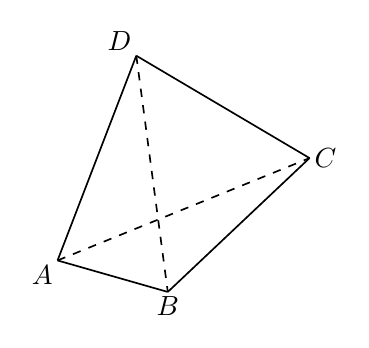
\begin{tikzpicture}[scale=1.0, semithick, every node/.style={inner sep=1.5pt}]
  \coordinate (D) at (2.0,3.2);
  \coordinate (A) at (1.0,0.6);
  \coordinate (C) at (4.2,1.9);
  \coordinate (B) at (2.4,0.2);
  \draw (D) -- (A);
  \draw (D) -- (C);
  \draw (C) -- (B);
  \draw (A) -- (B);
  \draw[dashed] (A) -- (C);
  \draw[dashed] (D) -- (B);
  \node[above left] at (D) {$D$};
  \node[below left] at (A) {$A$};
  \node[right] at (C) {$C$};
  \node[below] at (B) {$B$};
\end{tikzpicture}
